\section{Appendix B - Technical Notes}
\label{sec:Appendix_B}
\subsection{Normalisation}

One of the principal challenges in SONAR processing is that the underwater acoustic environment is highly dynamic. Background noise levels vary due to sea state, vessel traffic, marine life, weather conditions, and the motion of the sonar platform itself. As a result, detection algorithms must distinguish meaningful targets from continually changing acoustic backgrounds. To reduce the impact of this MACS uses a statistical technique called normalization. MACS's normalisation is enabled with a toggle (Section 3) with configurable parameters in the settings panel.

\subsubsection{What MACS does}

\textbf{The Process:} raw acoustic information is fed from MNW into MACS which then applies a Fast Fourier Transform (FFT) to convert the data from the time domain to the frequency domain. Sliding-window z-scores can then be computed for each frequency bin or beam direction. Each FFT value is compared with its local neighbourhood and converted into a z-score that measures how many standard deviations it lies above or below the local background level. If a particular frequency band suddenly exhibits energy that is significantly higher than its recent average, the resulting z-score will be increased relatively. Such behaviour may indicate the presence of a target, such as a submarine, underwater vehicle, or marine mammal. It is the relative differences that are then colour mapped to the LOFAR display. The process is summarized in Figure 22.

\begin{figure}[ht]
	\centering
	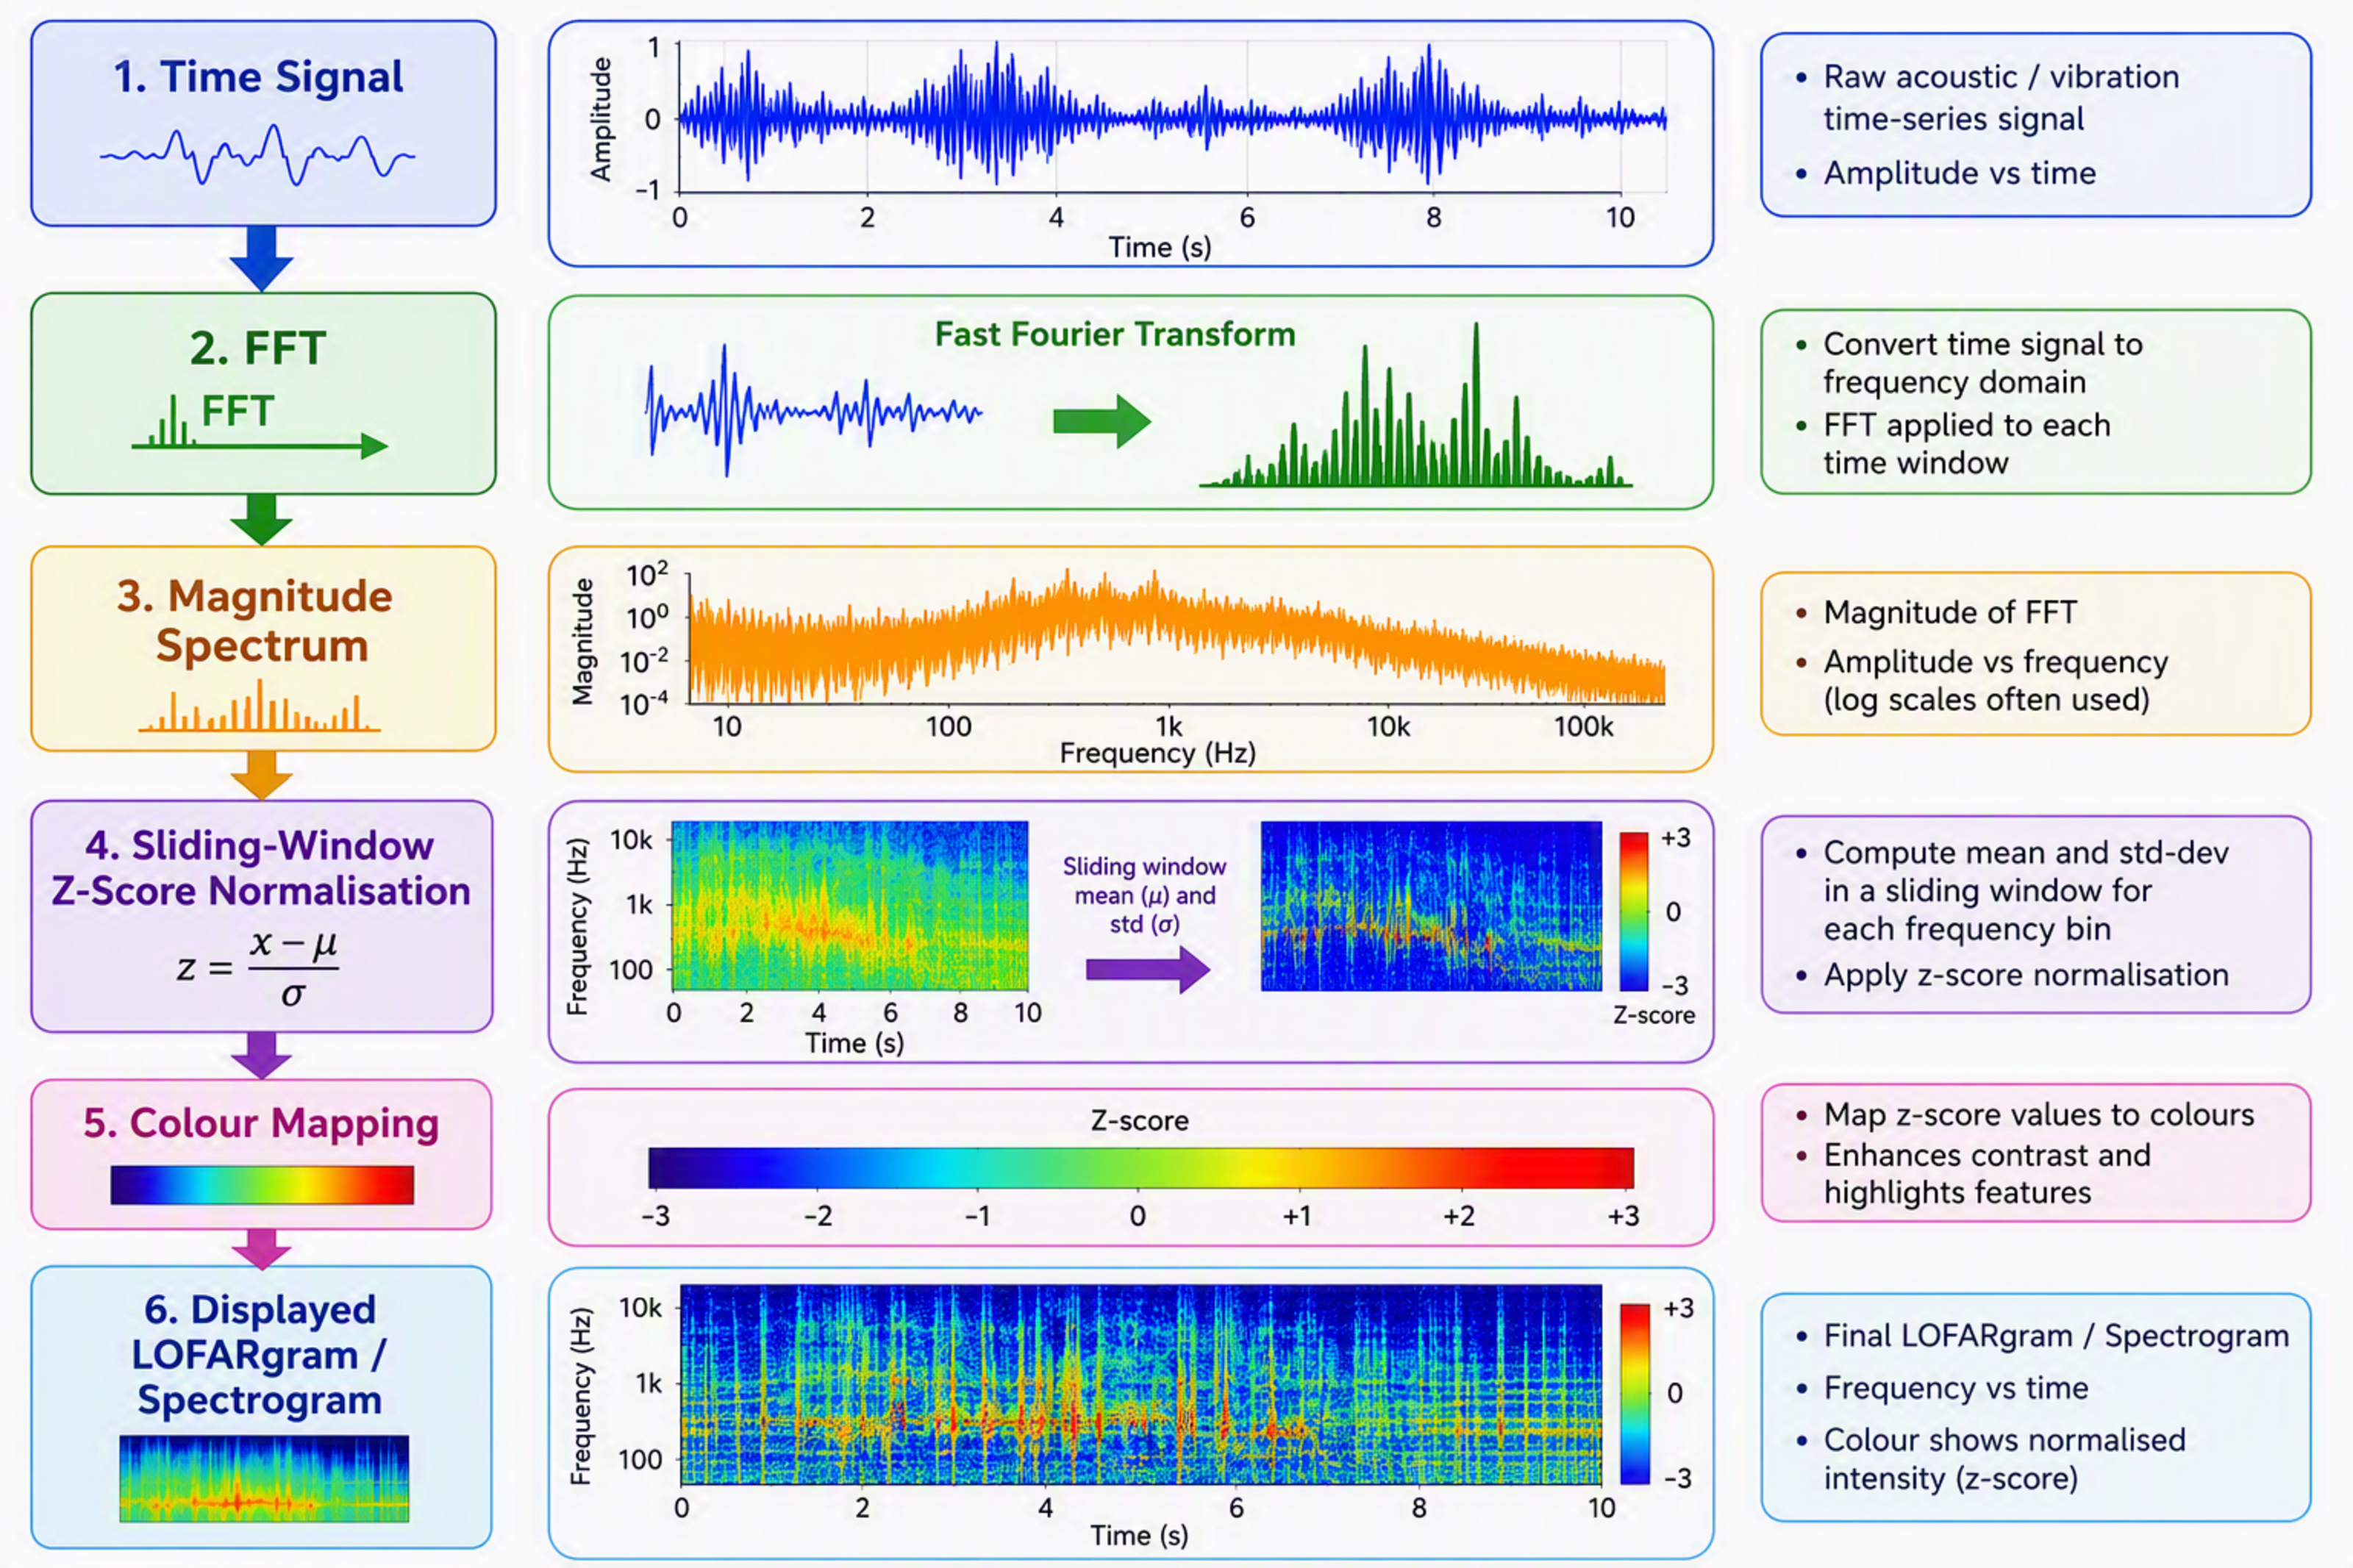
\includegraphics[width=400px]{../img/actuals/normalisation.pdf}
	\caption{FT from time domain to frequency domain}
\end{figure}


\textbf{Sliding window z-score:} is a statistical algorithm that measures how unusual a current observation is relative to recent observations (the window) rather than relative to the entire dataset. This means that the current observation is measured locally to its windowed set. The window slides along the data set as the analysis progresses. This adaptive normalisation continuously updates as new data arrive, allowing the detection process to remain sensitive even when the overall acoustic environment changes.

For a measured acoustic feature in each frequency bin the normaliser computes:

\[
z_{t} = \frac{x_{t} - \mu_{t}}{\sigma_{t}} \times \mathrm{Normalisation Output Scale}
\]

Where:
\begin{compactitem}
    \item $\mu_{t}$ is the mean computed over a recent time window (width controlled by Mean Half-Width see Parameters below).
    \item $\sigma_{t}$ is the standard deviation computed over across a potentially different sliding window (width controlled by Standard Deviation Half-Width see Parameters below).
    \item Normalisation Output Scale is a multiplier (range 1-50, default 20) that rescales z-scores into a range compatible with the Floor / Dynamic Range colour scale.
\end{compactitem}

% Both windows are computed efficiently using O(n) prefix sums -- no per-frame re-computation cost.

\subsubsection{MACS - LOFAR style example - from FFT to colour-mapping.}

The whole process is best explained with an simplified example. Given a set of raw FFT magnitudes, suppose one FFT frame contains these frequency bins:

 \begin{tabular}{ll}
    Frequency Hz & Magnitude \\
    \hline
    10 & 95 \\
    20 & 102 \\
    30 & 98 \\
    40 & 105 \\
    50 & 140 \\
    60 & 104 \\
    70 & 97 \\
    80 & 101\\
    90 & 99
 \end{tabular}

The 50 Hz bin (140) is suspected to be a machinery tone sitting above a background level of roughly 100. The question is, whether the difference between the tonal and background is significant. This is where MACS can assist by determining the significance and then visualise that.

Assume a window half-width of 2 bins which means the window always contains $2 \times 2 + 1 = 5$ bins (the centre value and two either side). For the first position the window is centred on Bin 3:

 \begin{tabular}{lllll}
    95 & 102 & 98 & 105 & 140 \\
    \hline
    1 & 2 & 3 & 4 & 5
 \end{tabular}

The algorithm calculates from those 5 values:
\begin{compactitem}
    \item Mean $\mu = 108$
    \item Standard deviation $\sigma = 16$
\end{compactitem}

Then it computes the z-score only for the centre bin (Bin 3).

\[
z_{3} = \frac{98 - 108}{16}
\]
\[
z_{3} = -0.63
\] 

Now the window slides right by one bin:

 \begin{tabular}{lllll}
    102 & 98 & 105 & 140 & 104 \\
    \hline
    2 & 3 & 4 & 5 & 6
 \end{tabular}

Now the centre is Bin 4. A completely new mean and standard deviation are calculated $\mu = 109.8$, $\sigma = 15.3$ resulting in $z_{4} = -0.31$
 
Window slides again

 \begin{tabular}{lllll}
    98 & 105 & 140 & 104 & 97 \\
    \hline
    3 & 4 & 5 & 6 & 7
 \end{tabular}

Now the centre is Bin 5, the machinery tone. $\mu = 108.8$, $\sigma = 15.9$ so $z_5 = 2.0$. The machinery line stands out because it is two standard deviations above the local background.

Continuing across the entire spectrum; the process repeats until every FFT bin has its own z-score.

 \begin{tabular}{llc}
    Bin & Magnitude & Z-Score \\
    \hline
    1 & 95 & -0.8\\
    2 & 102 & 0.1\\
    3 & 98 & -0.6\\
    4 & 105 & -0.3\\
    5 & 140 & 2.0\\
    6 & 104 & 0.1\\
    7 & 97 & -0.5\\
    8 & 101 & 0.0\\
    9 & 99 & -0.2
 \end{tabular}

Notice that the raw amplitudes have disappeared. Every bin is now expressed in terms of how unusual it is relative to its neighbours. The final step is mapping the z-scores to a colour map.

\begin{tabular}{ll}
    Z-Score & Colour \\
    \hline
    \verb|<| -1 & Dark Blue \\
    -1 to 0 & Blue \\
    0 to 1 & Green \\
    1 to 2 & Yellow \\
    2 to 3 & Orange \\
    \verb|>| 3 & Red
 \end{tabular}

This results in the following display where the 50 Hz machinery line now appears as a bright orange feature, distinct from the background.

 \begin{tabular}{lllcl}
    Bin & Frequency Hz & Magnitude & Z-Score & Color\\
    \hline
    1 & 10 & 95 & -0.8 & Blue\\
    2 & 20 & 102 & 0.1 & Green\\
    3 & 30 & 98 & -0.6 & Blue\\
    4 & 40 & 105 & -0.3 & Blue\\
    5 & 50 & 140 & 2.0 & Orange\\
    6 & 60 & 104 & 0.1 & Green\\
    7 & 70 & 97 & -0.5 & Blue\\
    8 & 80 & 101 & 0.0 & Blue\\
    9 & 90 & 99 & -0.2 & Blue
 \end{tabular}

Suppose another region of the spectrum looks like this:

\begin{tabular}{ll}
    Frequency Hz & Magnitude \\
    \hline
    500	& 20 \\
    510	& 21 \\
    520	& 20 \\
    530	& 26 \\
    540	& 19
\end{tabular}

The standout tone at 530 Hz is only 26 magnitude, which seems tiny compared with the 140 at 50 Hz but the local mean $\approx 21$ and the local standard deviation $\approx 2$ gives $z = \frac{26-21}{2} = 2.5$. This second tone gets a higher z-score than the 50 Hz one so in the final LOFARgram it may actually appear brighter, because it is more unusual relative to its local noise environment.

\begin{faintquote}
    That is the key idea behind the statement: "The algorithm used is a sliding-window z-score of the FFT magnitude output before colour mapping." The colours no longer represent absolute acoustic energy. They represent how significant each FFT bin is relative to its local background.
\end{faintquote}

Several example spreadsheets are provided for this process in the Spreadsheets folder at the \href{https://github.com/nbowling/MACS_Guide_Working}{GitHub repository} for this document.

\subsubsection{Adjustment Parameters via the Setting Panel}

MACS has sensible defaults for the key normalisation parameters however there are times when you would want to fine tune them. Turn on normalisation by ticking the option box on the LOFAR panel then clicking settings $\rightarrow$ Analysis Defaults tab. The normalisation settings are at the bottom of the panel.

\begin{compactenum}
    \item \textbf{Mean Width:} Sliding window half-width (in frames) used to compute the local mean. Wider $\rightarrow$ slower adaptation to changing noise level.
    \item \textbf{StdDev Width:} Sliding window half-width for standard deviation. Can differ from Mean Width. If $\sigma > 2  \times \mu$, the noise floor is highly non-stationary.
    \item \textbf{Output Scale:} Multiplies all z-scores before colour mapping. Increase if the waterfall is too dim, decrease if it saturates. Start around 20 and adjust by eye.
\end{compactenum}

It is difficult to give exact advice for the best settings because they are very situation dependent, in general:

\begin{compactenum}
    \item Short mean window $\rightarrow$ remove local background variations and slow trends.
	\item Long standard-deviation window $\rightarrow$ estimate the ambient noise floor robustly.
\end{compactenum}

This tends to make narrowband machinery tones and transient features more visible without allowing them to significantly affect the variance estimate.

As a general rule of thumb the following table gives basic usage:

\begin{tabular}{ll}
    Window size	& Effect \\
    \hline
    Very small & Highly adaptive, noisy normalisation \\
    Moderate & Good compromise \\
    Very large & Stable statistics, less adaptive \\
    Mean window \verb|<| Std-dev window & Common and often desirable \\
    Mean window $\approx$ Std-dev window & Standard sliding z-score \\
    Std-dev window too small & Can suppress strong events
\end{tabular}

A useful way to think about it is:
\begin{compactitem}
	\item Mean window controls how quickly the baseline can move.
	\item Std-dev window controls what the algorithm considers to be the "normal" noise level.
\end{compactitem}

For LOFAR or spectrogram preprocessing, the standard-deviation window is often chosen several times larger than the mean window so that transient or tonal features remain prominent after normalisation.

\begin{faintquote}
    Consider a passive SONAR system monitoring vessel noise. The background acoustic level may gradually increase as ocean conditions change during the day. A conventional threshold based on absolute signal level might generate numerous false alarms or miss weak targets. In contrast, a sliding-window z-score compares the current observation with the local acoustic environment. A ship propeller tone that rises above the recent background will produce a large positive z-score, making it easier to detect even when absolute noise levels are elevated. This adaptive normalisation continuously updates as new data arrive, allowing the detection process to remain sensitive even when the overall acoustic environment changes.

    \begin{compactenum}
        \item \textbf{Suppresses slowly varying broadband noise:} bins that are consistently loud have a high mean, which gets subtracted. What remains is deviations from the local average.
        \item \textbf{Enhances tonal lines:} a persistent narrowband tone will have a value consistently above its local mean, showing up as a bright persistent line even against a noisy background.
        \item \textbf{The z-score can go negative} (a bin quieter than average). The Floor control clips these to the background colour.
    \end{compactenum}
\end{faintquote}

\subsubsection{When to use}

Enable normalisation when the background noise level is high and tonal lines are hard to see. It is particularly effective when the ship is manoeuvring and the broadband level is changing; the local mean tracks the change and removes it. Disable it for clean recordings where tonals are already visible, or when you need absolute amplitude information for noise reference subtraction.
\begin{faintquote}
    In summary. Sliding-window z-score normalisation converts raw SONAR measurements into a measure of statistical deviation from the recent acoustic background, enabling robust target detection in noisy underwater environments.
\end{faintquote}

\subsection{Fourier Transform}
\subsubsection{Introduction}

Many things that vary over time or space appear complicated when viewed directly: a piece of music, a seismic tremor, a photograph, a radio transmission, or even fluctuations in financial data. The Fourier Transform (FT) offers a markedly different perspective. Instead of asking, “What is this signal doing at each moment?” it asks, “Which frequencies combine to create it?”

Named after the French mathematician Joseph Fourier (1768-1830), the transform originated from his work on heat conduction. Today it is one of the most important mathematical tools in science and engineering, fundamental to fields ranging from physics and telecommunications to medical imaging and machine learning. At its core, it is a mathematical microscope that peers into complex, messy signals and extracts the fundamental building blocks: pure frequencies. Whether studying sound waves, radar signals, vibration measurements, electrical systems, or digital communications, the FT provides a powerful way to understand how energy is distributed across different frequencies.

\subsubsection{From waves to ingredients an analogy: Unmixing the Smoothie}

An often used analogy for FT is to imagine making a fruit smoothie. Once blended, you have a single, uniform liquid. If someone asked you to measure the exact amount of strawberries, bananas, and milk in that finished glass, it would be almost impossible just by looking at it.

Two terms that commonly appear are \enquote{Time Domain} and \enquote{Frequency Domain}. Using our smoothie they can be explained in the following way:

\begin{compactitem}
    \item The Time Domain is the smoothie itself — the raw, combined signal as it exists in the real world over time.
    \item The Fourier Transform is the magic machine that takes the finished smoothie and separates it back into individual piles of fruit.
    \item The Frequency Domain is the recipe — the broken-down smoothie showing exactly how much of each ingredient (frequency) makes up the whole (Figure 23).
\end{compactitem}

\begin{figure}[ht]
	\centering
	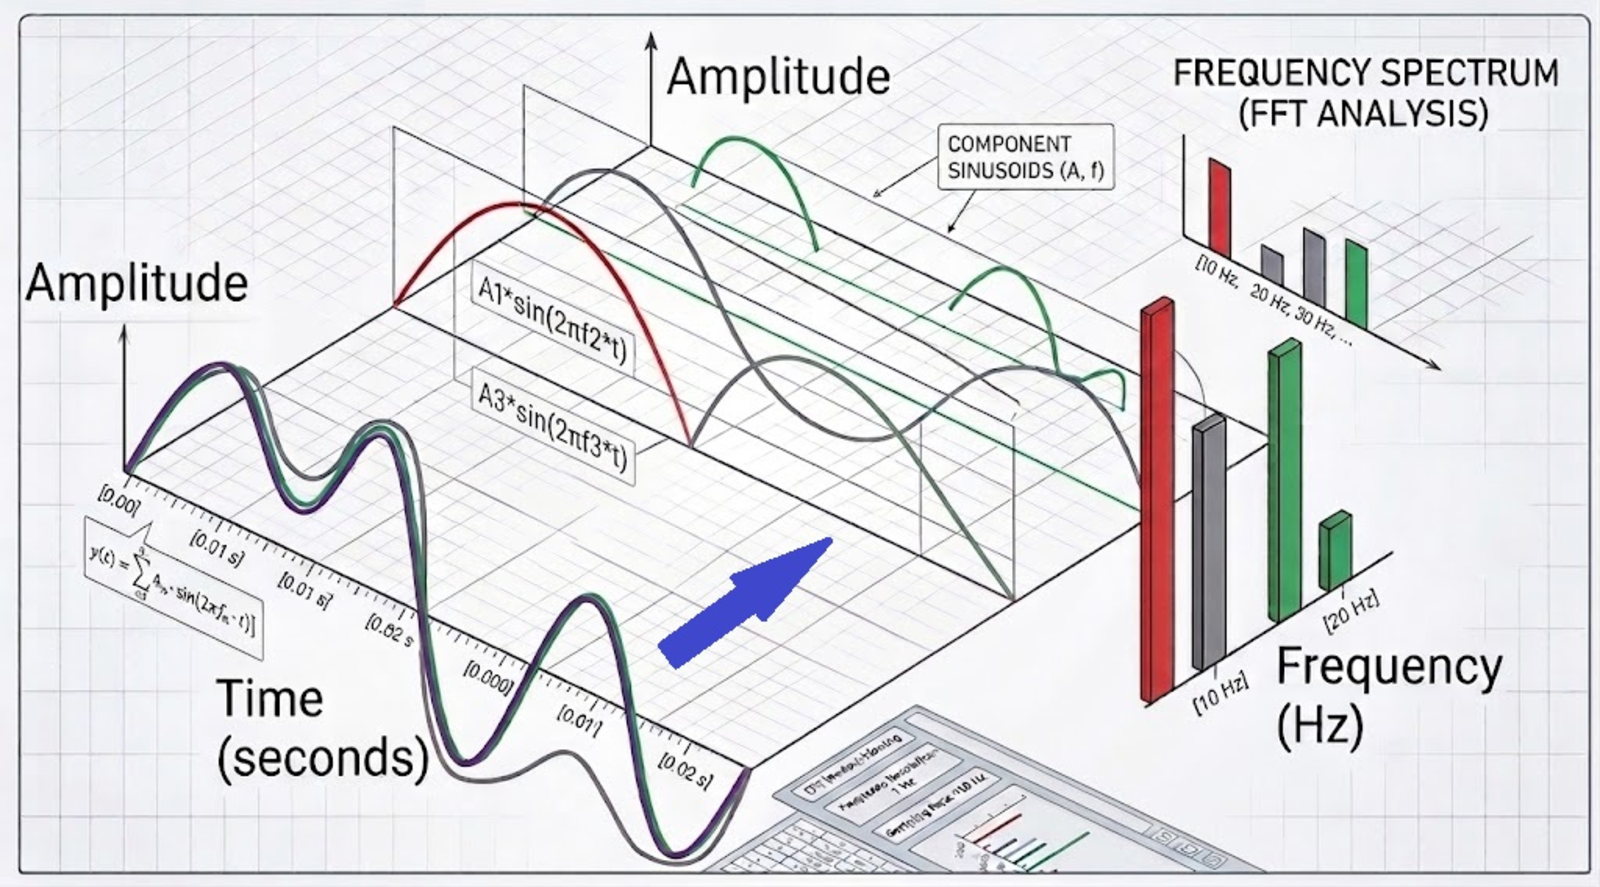
\includegraphics[width=300px]{../img/actuals/TD2FD.pdf}
	\caption{FT from time domain to frequency domain}
\end{figure}

\begin{faintquote}
    A signal can be represented in two complementary ways:
    \begin{compactitem}
        \item The time domain shows how it changes over time.
        \item The frequency domain shows the strength of its component frequencies.
    \end{compactitem}
\end{faintquote}

\subsubsection{Why is it relevant to me}

In underwater acoustic analysis, passive sonar techniques used by submarines and surface ships to detect, classify, and track underwater targets (like submarines, surface vessels, or torpedoes) rely on the FT, it is the core mathematical engine that makes LOFAR, DEMON and other sonar processing tools work. Undersea targets produce a complex mix of continuous broadband noise (water displacement, turbulent flow) and discrete narrowband tonal signals (machinery, engine vibrations, propeller blade passage). The FT isolates these hidden narrowband tonals from background ocean noise.

\begin{compactitem}
    \item Short-Time Fourier Transform (STFT): Hydrophones continually record continuous time-domain voltage/acoustic signals $f(t)$. Because underwater sound changes over time, the signal is chopped into overlapping time windows (slices), and an FT is computed for each window.
    \item Creating the "Lofargram" (Waterfall Display): The magnitude of each FT frame becomes a single row of pixels, where the x-axis represents Frequency, colour/brightness represents Signal Energy (dB), and the Y-axis scrolls downward representing Time.
\end{compactitem}


Key Applications of FT in LOFAR Analysis

\begin{compactenum}
    \item Target Classification and Fingerprinting:
    \begin{compactitem}
        \item Rotating propellers, reduction gears, onboard generators, and cooling pumps vibrate at precise frequencies.
        \item The FT isolates these frequencies as sharp vertical lines (tonals) on the Lofargram. Sonar operators match these line patterns against acoustic libraries to identify the exact class or ship name of a vessel miles away.
    \end{compactitem}
    \item Measuring Shaft/Blade RPM:
    \begin{compactitem}
        \item Propeller cavitation produces fundamental frequencies and harmonics. By applying the Fourier Transform, operators can calculate propeller blade counts and shaft rotation speeds (RPM) to determine target speed.
    \end{compactitem}
    \item Enhancing Signal-to-Noise Ratio (SNR):
    \begin{compactitem}
        \item Ocean background noise spreads across a wide band of frequencies. By running long FFT integration times (narrow frequency bins), the power of a single steady mechanical tone concentrates into a single frequency bin, making faint targets stand out clearly above the background noise.
    \end{compactitem}
\end{compactenum}


\subsubsection{The Basic Idea and Mathematical Definition}

Arguably, the FT is one of the most elegant and practical mathematical concepts ever devised although much credit must go to Euler who's insight was the starting point for Fourier.

The basic premise is that any periodic signal can be represented as a sum of sine and cosine waves of different frequencies, amplitudes, and phases.

\begin{compactitem}
    \item Frequency: How fast the wave repeats itself, measured as the number of complete cycles per second (Hertz, or Hz). Higher frequency means more rapid oscillations (e.g., a higher pitch in sound or higher speed in rotation).
    \item Amplitude: The height or strength of the wave, measured as the distance from its rest position to its highest peak. Higher amplitude means greater power or intensity (e.g., a louder sound or a higher peak voltage).
    \item Phase: The timing or relative position of a wave within its cycle at a specific starting point, measured in degrees ($0^\circ$  to $360^\circ$) or radians (0 to $2\pi$). If two waves are "in phase," their peaks align at the same time; if they are "out of phase," one is shifted horizontally relative to the other.
\end{compactitem}

For example, a square wave can be approximated by:
\[
    x(t)=sin(\omega t) + \frac{1}{3} sin(3\omega t) + \frac{1}{5}sin(5\omega t) + ...
\]
The symbol $\omega$ represents angular frequency and is closely related to ordinary frequency $f$, measured in cycles per second or Hertz (Hz)
\[
    \omega=2\pi f
\]
Where:
\[
\begin{aligned}
    \omega &= \text{angular frequency (radians per second)}  \\
    f &= \text{frequency (Hz)} \\
    2\pi &= \text{radians in one complete cycle}
\end{aligned}
\]

Although the square wave looks totally different from a sine wave, it can be constructed by adding together many sinusoidal components. The FT generalizes this concept to arbitrary signals.

For a continuous-time signal the Fourier Transform is defined as:
\[
    \hat{f}(\xi)=\int\limits_{-\infty}^\infty f (t) e^{-j2\pi \xi t}\,dt
\]
The inverse Fourier Transform reconstructs the original signal:
\[
    f(t)=\int\limits_{-\infty}^\infty X (\xi) e^{j2\pi \xi t}\,dt
\]

These equations show that the time and frequency domains contain equivalent information.

Where:
\begin{align*}
    f(t) &\quad\text{--}\quad \parbox[t]{12cm}{\raggedright \textbf{The Input Signal:} The original time-domain signal (e.g., sound pressure over time or a changing voltage).} \\[1.5ex]
    \xi &\quad\text{--}\quad \parbox[t]{12cm}{\raggedright \textbf{The Target Frequency:} The specific probe frequency being tested. The equation evaluates one value of $\xi$ at a time.} \\[1.5ex]
    e^{-j2\pi \xi t} &\quad\text{--}\quad \parbox[t]{12cm}{\raggedright \textbf{The Complex Rotator:} By Euler's identity ($e^{jx}=\cos x + j \sin x$), this term represents a point rotating around a unit circle in the complex plane at frequency $\xi$. The negative sign causes clockwise rotation.} \\[1.5ex]
    f(t)\cdot e^{-j2\pi \xi t} &\quad\text{--}\quad \parbox[t]{12cm}{\raggedright \textbf{The Signal Winding:} Multiplying the original signal $f(t)$ by this rotating complex exponential wraps the 1D signal into a 2D spiral in the complex plane.} \\[0.75ex]
    \int\limits_{-\infty}^{\infty} &\quad\text{--}\quad \parbox[t]{12cm}{\raggedright \textbf{Finding the Center of Mass:} Integrating sums up all the points on that spiral over all time.}
\end{align*}

\textbf{The Mechanical Intuition: "Winding" the Signal}

To visualize how the integration extracts a frequency, imagine wrapping a physical audio signal line around a circle at a variable winding rate:
\begin{compactenum}
    \item Unmatched Frequency ($\xi \ne$ signal frequency): The spiral winds unevenly. Points spread evenly around the center in all directions, causing positive and negative values to cancel out. The integral evaluates to roughly zero.
    \item Matched Frequency ($\xi =$ signal frequency): The signal's peaks line up on one side of the circle, pulling the entire spiral off-center. The integral sums these aligned values, resulting in a large spike.
\end{compactenum}

The final output, $\hat{f}(\xi)$, is a complex number where the magnitude represents the strength of that frequency in the signal, and the angle (phase) indicates how that frequency aligns in time. While magnitude often receives the most attention, phase is essential for accurately reconstructing the original waveform.

Suppose a signal contains:
\[
    x(t) = 3 \sin( 2 \pi 50 t) + 2 \sin(2 \pi 120 t) \quad \text{(Figure 24)}
\]

 \begin{figure}[ht]
	\centering
	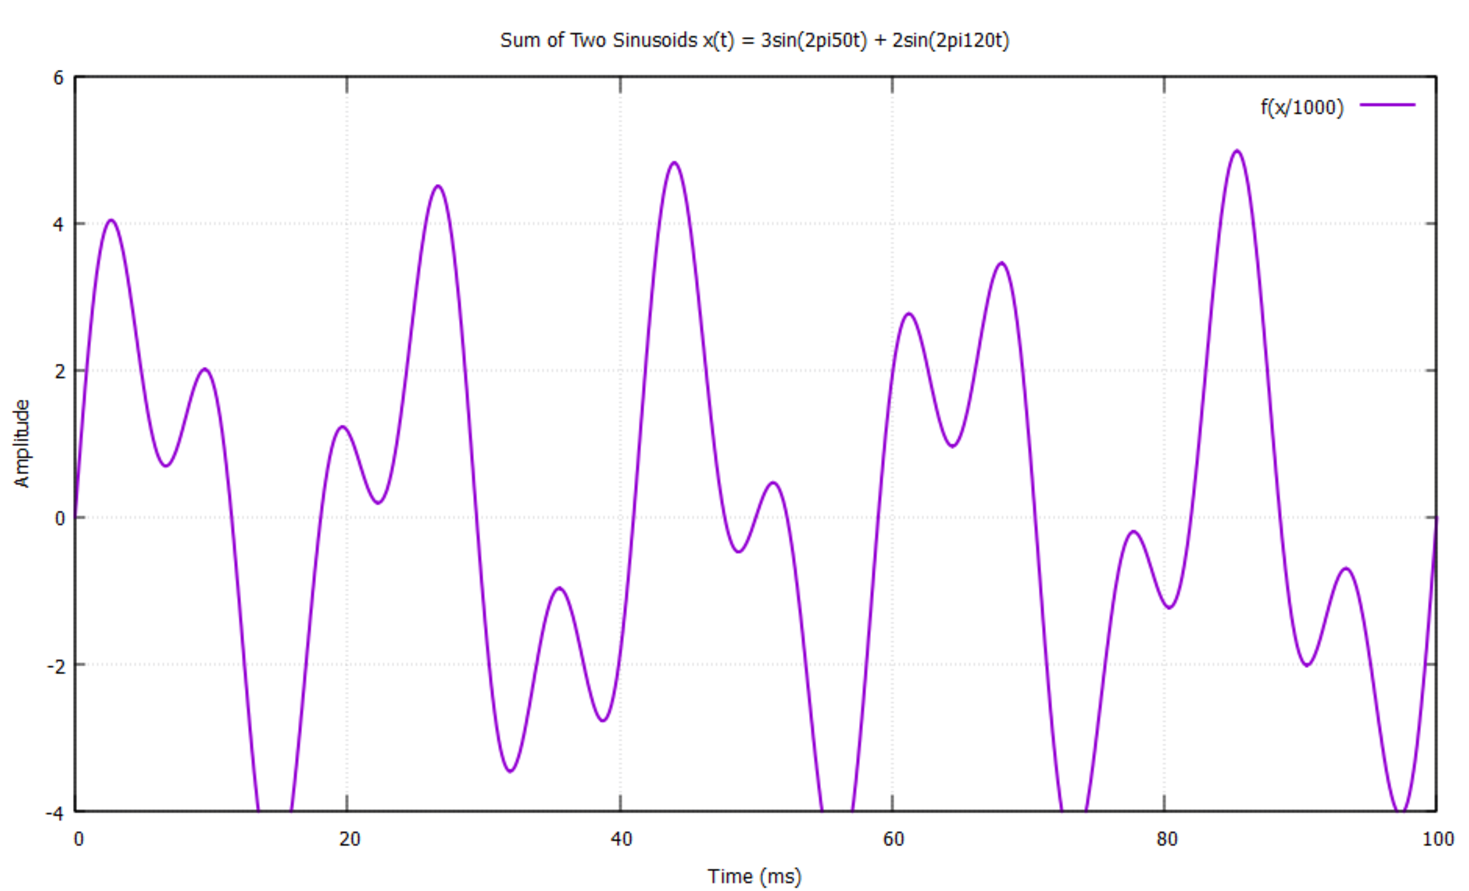
\includegraphics[width=300px]{../img/actuals/CmplxWave.pdf}
	\caption{Complex wave function}
\end{figure}

Visually, the waveform is complicated, but after applying the FT, two clear peaks appear; the transform immediately reveals the signal's composition.

 \begin{tabular}{lc}
    Frequency & Amplitude \\
    \hline
    50 Hz & 3 \\
    120 Hz & 2
 \end{tabular}

\subsubsection{Discrete Fourier Transform (DFT) and Fast Fourier Transform (FFT)}
Real-world measurements are sampled digitally. Consequently, computers use the Discrete Fourier Transform (DFT) rather than the continuous FT. The DFT converts sampled data into discrete frequency bins.

For a sequence containing N samples:
\[
 X[k]=\sum_{n=0}^{N-1}x [n] e^{-j2\pi kn/N}
\]
However the DFT can be computationally expensive for large datasets.  Instead modern analysts use the FFT algorithm to compute the DFT. The FFT is most commonly associated with James Cooley and John Tukey, who published the famous Cooley-Tukey FFT algorithm in 1965. Their paper showed how to compute a Discrete Fourier Transform much more efficiently, reducing the computational effort from roughly $O(N^2)$ operations to $O(N\log_{10} N)$. For a million-sample signal, the FFT may perform thousands of times faster than a direct DFT calculation.

\subsubsection{In terms of Marine Acoustics: A Concrete Audio Example}

In underwater passive sonar, a classic task is calculating the Blade Pass Frequency (BPF) of a submarine's propeller using a LOFARgram (direct spectrum analysis) and a DEMON spectrum (demodulation envelope analysis). Below is a complete numerical example demonstrating how a sonar signal processor converts raw acoustic line frequencies into target speed and machinery specifications.

\textbf{Scenario \& Given Data}

A passive sonar hydrophone array detects a contact. The signal processing pipeline in MACS generates two spectral plots from the sound recording:

\begin{compactenum}
    \item LOFAR Spectrum: Displays a strong, fundamental machinery tonal line at $f_{tonal} = 120 Hz$.
    \item DEMON Spectrum: Displays an envelope modulation spectrum with distinct harmonic peaks at 5 Hz, 10 Hz, 15 Hz, and 20 Hz".
\end{compactenum}

From intelligence database records, this target class is known to use a 7-bladed propeller ($N_{blades} = 7$) with a pitch (P) of 8 feet per revolution and a known slip (S) of 15\verb|%| (Efficiency Factor = $1 - 0.15 = 0.85$).

\textbf{Step-by-Step Numerical Analysis}
\begin{compactenum}
    \item \textbf{Determine the Fundamental Shaft Frequency (SR):}
        \begin{compactenum}[i]
            \item In the DEMON spectrum, the periodic mechanical modulation of propeller cavitation produces peaks at fundamental rotation rates and their harmonics.
            \item The lowest fundamental peak in the envelope spectrum represents the Shaft Fundamental (SF).
            \item $SF = 5$ Hz
        \end{compactenum}
    \item \textbf{Calculate Propeller Shaft Speed (SR in RPM):}
        \begin{compactenum}[i]
            \item To convert the shaft fundamental from Hertz (revolutions per second) to Shaft Rate (SR) in Revolutions Per Minute (RPM)
            \item $SR = SF \times 60$ $\rightarrow$  $5 \times 60 = 300$ RPM
        \end{compactenum}
    \item \textbf{Calculate the Blade Rate (BR):}
        \begin{compactenum}[i]
            \item The Blade Pass Frequency is the rate at which individual propeller blades pass a fixed point. It is the product of the shaft frequency and the number of blades
            \item $BPF=SF \times N_{blades} \rightarrow 5 \times 7 = 35$ Hz
            \item On a LOFARgram or DEMON spectrum, a peak would appear right at 35 Hz
        \end{compactenum}
    \item \textbf{Identify Machinery Gear Ratio from LOFAR Tonal:}
        \begin{compactenum}[i]
            \item Now we link the DEMON results back to the LOFAR spectrum tonal line ($f_{tonal} = 120$ Hz).
            \item If this tonal line is generated by a diesel engine or reduction gear driving the main shaft, we can calculate the exact gear/vibration ratio (R) relative to the shaft turn
            \item $R = \frac{f_{tonal}}{SF} \rightarrow \frac{120}{5} = 24$
            \item This tells the sonar analyst that the machinery generating the 120 Hz tone turns at 24 times the rate of the main propeller shaft ($24 \times 300 = 7,200 RPM$).
        \end{compactenum}
\end{compactenum}

\textbf{Theoretical Speed} if no propeller slip.

\begin{compactenum}
    \item Distance per minute = $SR \times P$ = $300 \times 8 = 2,400$ ft/min
    \item Distance per hour = $2,400 \times 60$ = 144,000 ft/hr $\rightarrow$ $\frac{144,000}{6076} \approx$ \underline{23.7 Knots/hr} (6076 ft/nautical mile)
\end{compactenum}

\textbf{Speed accounting for propeller slip}

\begin{compactenum}
    \item $\text{Theoretical Speed} \times (1 - S)$
    \item $23.7 \times (1 - 0.15) = 23.7 \times 0.85 \approx$ \underline{20.1 Knots / hr}
\end{compactenum}

Both steps can be combined in one formula:

\[
    \text{Speed (Knots)} = \frac{SR \times P \times ( 1 - S)}{6076}
\]

\textbf{Summary of Results}

\begin{tabular}{lll}
    Parameter & Formula & Calculated Value \\
    \hline
    Shaft Frequency (SF) & Primary DEMON peak & 5.0 Hz \\
    Shaft Rate & $SF \times 60$ & 300 RPM \\
    Blade Pass Frequency (BPF)	& $SF \times N_{blades}$ & 35 Hz \\
    Machinery Gear Ratio & $f_{tonal}/SF$ & 24:1 \\
    Speed through water & $\text{Speed (Knots)} = \frac{SR \times P \times (1 - S)}{6076}$ & 20.1 Kts/hr
\end{tabular}

By performing these steps, a passive sonar operator confirms not only the target's operating speed, but also verifies the contact's identity against known propeller and engine drive signatures.

\subsubsection{Limitations}
A standard Fourier Transform tells us which frequencies exist in a signal, but not always when they occur. If a song changes from a bass note to a violin note, the overall transform identifies both frequencies but does not precisely mark their timing.

These limitations are the reason other techniques such as the Short-Time Fourier Transform, spectrograms, wavelets, and order tracking were developed. For many marine acoustic problems, a spectrogram (successive FFTs over time) is often more informative than a single Fourier Transform because it reveals how shaft-rate, blade-pass, and cavitation frequencies evolve as vessel speed changes.

There is also a fundamental trade-off: greater precision in time generally comes at the cost of precision in frequency, and vice versa. This relationship is closely related to the uncertainty principle in physics.

\subsubsection{Conclusion}
The Fourier Transform is a cornerstone of modern science and engineering. By converting signals from the time domain to the frequency domain, it reveals information that is often hidden in raw measurements. Its digital implementation through the Discrete Fourier Transform and Fast Fourier Transform enables practical analysis of everything from music and radio transmissions to vibration measurements and underwater acoustics. As a result, the Fourier Transform remains one of the most widely used mathematical techniques for understanding, analysing, and processing complex signals.

\subsection{LOFAR}
\textcolor{commentGreen}{*** WIP ***}

What it is: A standard acoustic spectrogram displayed as a waterfall. Each new FFT frame is added as a horizontal line of pixels scrolling bottom to top; the horizontal axis is frequency; colour encodes amplitude in dB. Persistent vertical lines marching across the display indicate tonal components — discrete narrowband signals that stand out from the broadband noise background.

\textbf{Signal path:}

\begin{compactenum}
    \item Audio samples arrive from the engine (live or file playback).
    \item An optional bandpass filter is applied.
    \item An optional noise reference is subtracted.
    \item Samples are accumulated in an overlap buffer.
    \item An FFT is computed with zero-padding to match the display pixel width.
    \item Magnitudes are converted to dB.
    \item Optional normalisation is applied.
    \item The result is mapped through the Floor / Dynamic Range colour scale and painted as one column.
\end{compactenum}

\textbf{Key parameters:} FFT Size, Overlap, Floor, Dynamic Range, Normalisation, $F_{min}$ / $F_{max}$ display limits.

\subsection{DEMON}
\textcolor{commentGreen}{*** WIP ***}

\textbf{What it is:} DEMON (Detection of Envelope Modulation ON Noise) extracts the low-frequency modulation imposed on broadband acoustic noise by a vessel's rotating machinery (primarily propeller shaft and blade-rate harmonics). The result is a second spectrogram whose frequency axis covers 0 - $F_{max}$ Hz (typically 0 - 50 Hz), revealing shaft rotation rates and blade rates that are far too low to appear in the LOFARgram.

\textbf{Signal path:}

\begin{compactenum}
    \item Samples are bandpass-filtered to the selected DEMON band.
    \item The amplitude envelope is extracted using a 63-tap Type III linear-phase Hilbert FIR filter (Hann-windowed). This produces a clean, phase-correct envelope signal without the DC bias of simple rectification.
    \item The envelope is decimated by a factor computed as $\max(\frac{Fs}{(2 \times F_{max-demon})}, 1)$, floored by Nyquist and ceilinged by FFT resolution requirements. This dynamically sets the decimated sample rate just high enough to represent the DEMON band without wasting computation.
    \item An FFT is computed on the decimated envelope using the DEMON FFT size and overlap.
    \item The result is displayed as a waterfall, with the same Floor / Dynamic Range colour scale.
\end{compactenum}

 \begin{figure}[ht]
	\centering
	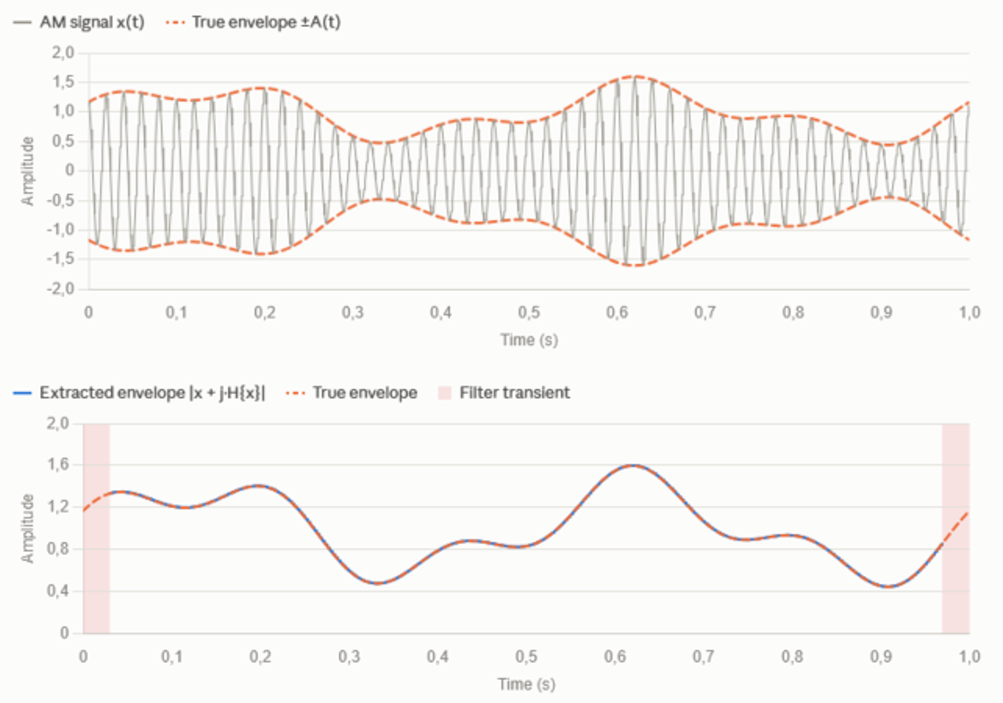
\includegraphics[width=300px]{../img/actuals/DEMONchart.pdf}
	\caption{DEMON process}
\end{figure}

\textbf{Why this works:} Rotating machinery amplitude-modulates the broadband acoustic noise it generates. For propeller-driven vessels, propeller blades periodically interrupt the cavitation noise; for diesel-engined vessels, piston firing events modulate the radiated noise at crankshaft rate and its harmonics. DEMON demodulates this carrier to make those low frequencies directly visible. It is effective for both propeller shaft / blade-rate detection (surface ships, submarines underway) and diesel engine firing rate detection (diesel-electric submarines at low speed).



\textbf{Key parameters:} DEMON band sets the acoustic carrier band to demodulate, DEMON Display Max ($F_{max}$ of the DEMON output display axis), DEMON FFT Size, Overlap, Floor, Dynamic Range.

\subsection{Cepstrum}
\textcolor{commentGreen}{*** WIP ***}

\textbf{What it is:} The real cepstrum is computed as:

\[
C(\tau) = \mathrm{IFFT}\{\log |X(f)|\}
\]

where X(f) is the FFT of the input signal and the log is of the \textbf{linear magnitude} (not dB - log is applied once inside the cepstrum formula). The result is plotted with the horizontal axis in quefrency (milliseconds), which is the reciprocal-domain equivalent of frequency.

A peak at quefrency $\tau$ ms indicates a strongly periodic structure with period $\tau$ ms in the spectrum - i.e., a family of harmonics spaced $1/\tau$ Hz apart. This makes the cepstrum particularly good at detecting harmonic combs even when individual harmonics are weak.

\textbf{Key parameters:} FFT Size (same as LOFARgram), Overlap, Floor, Dynamic Range. The quefrency axis runs from 0 to FFT Size / (2 x Fs) ms.

\textbf{Note on axis:} The cursor label reads `ms' (quefrency), not `Hz'. A peak at 20 ms corresponds to a fundamental period of 20 ms $\rightarrow$ fundamental frequency of 50 Hz.

\subsection{ACF}
\textcolor{commentGreen}{*** WIP ***}

\textbf{What it is:} The running autocorrelation function, computed via the Wiener–Khinchin theorem:

\[
R_{xx}(\tau) = \mathrm{IFFT}\{ |X(f)|^2\}
\]

The power spectral density is computed from the FFT, and its IFFT gives the autocorrelation. The horizontal axis is lag $(\tau)$, in milliseconds. A peak at lag $\tau$ ms means the signal is significantly self-similar at that delay — another indicator of periodicity. Unlike the cepstrum, the ACF does not take a logarithm, so it is more sensitive to dominant tones and less effective at compressing the dynamic range of a harmonic comb. Used together, cepstrum and ACF give complementary views of the same periodicity structure.

\textbf{Key parameters:} Same FFT Size and Overlap as the main pipeline. Floor / Dynamic Range colour scale.

\subsection{Noise Reference Subtraction}
\textcolor{commentGreen}{*** WIP ***}

Noise reference subtraction removes a pre-recorded background spectrum from the current signal, reducing stationary ambient noise.

\subsubsection{How it works}

The formula applied per frequency bin is:

\[
P_{clean(f)} = max( P_{signal(f)} - \alpha \times P_{noise(f)}, \beta \times P_{noise(f)} )
\]

\begin{compactitem}
\item $P_{signal(f)}$ is the current frame's power spectrum.
\item $P_{noise(f)}$ is the reference background spectrum (average of a selected reference recording).
\item $\alpha$ is the subtraction factor (typically 1.0 = full subtraction; increase to over-subtract and suppress more noise).
\item $\beta$ is a floor factor preventing the subtracted result from going below a fraction of the noise level (avoids musical noise artefacts).
\end{compactitem}

\subsubsection{Reference recording selection}
\begin{compactenum}
\item In the Recordings panel, select a WAV file that contains \textbf{only ambient/background noise} --- no contact of interest.
\item The file must be at least \textbf{15 seconds long} (enforced by validation). Short files produce unstable spectral averages.
\item Check the \textbf{``Use as noise reference''} checkbox next to that recording. Only one reference can be active at a time (exclusive selection --- checking one unchecks any previous reference).
\item Click \textbf{Load background} to compute and store the reference spectrum.
\end{compactenum}

\subsubsection{Effect}

Bins that are consistently present in the background (propulsion noise of your own vessel, ambient ocean noise, equipment self-noise) are attenuated. Signals from the contact --- which were not present in the background recording --- survive the subtraction and become more visible.

\subsubsection{Caveats}
\begin{compactitem}
\item The background must be representative of the noise during the analysis period. If own-ship speed or sea state changes significantly, the reference becomes stale.
\item Aggressive subtraction (high $\alpha$) can create musical noise --- random bright pixels where noise subtraction overshoots. Reduce $\alpha$ or adjust the floor factor if this occurs.
\item Normalisation and noise reference subtraction can be used together, but experiment --- they address different aspects of the noise problem (non-stationary broadband vs stationary background).
\end{compactitem}

\subsection{Power Density Spectral Analysis}
\textcolor{commentGreen}{*** WIP ***}

\subsection{ZOOMfft}
\textcolor{commentGreen}{*** WIP ***}

\pagebreak